\documentclass{standalone}

\usepackage{tikz}
\usetikzlibrary{shapes, arrows}
\usetikzlibrary{arrows,calc,decorations.markings,math,arrows.meta}
\usetikzlibrary{positioning}
\usepackage{graphicx}
\usepackage{adjustbox}
\usepackage{calc}




\begin{document}
\trimbox{-0.3cm -0.3cm -0.3cm -0.3cm}{ 
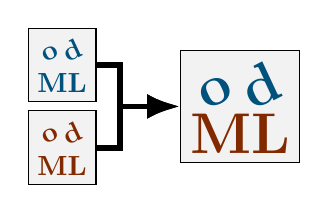
\begin{tikzpicture}

		    \definecolor{odmlcolor}{rgb}{0.00,0.32,0.49}
		    \definecolor{compcolor}{rgb}{0.51,0.16,0.00}
		    \definecolor{back}{rgb}{0.95,0.95,0.95}
% 		    \definecolor{color1}{rgb}{}
		    \node(odml1) [draw,align=center,font=\bfseries,preaction={fill, back}]{\textcolor{odmlcolor}{\rotatebox[origin=c]{25}{o}\rotatebox[origin=c]{25}{d}} \\ {\textcolor{odmlcolor}{ML}}};
		    \node(odml2) [below=.1cm of odml1,draw,align=center,font=\bfseries,preaction={fill, back}]{ \textcolor{compcolor}{\rotatebox[origin=c]{25}{o}\rotatebox[origin=c]{25}{d}} \\ {\textcolor{compcolor}{ML}}};
		    
		    \node(odml3) [right=1.5cm of $(odml1)!0.5!(odml2)$,draw,align=center,font=\bfseries,preaction={fill, back}]{\huge \rotatebox[origin=c]{25}{\textcolor{odmlcolor}{o}}\rotatebox[origin=c]{25}{\textcolor{odmlcolor}{d}}\\
												         \huge \textcolor{compcolor}{M}\textcolor{compcolor}{L}};
												         
		    
		    \draw[-{Latex[scale=1]},line width=0.7mm] (odml1.east) -- ++(0.3,0) |- (odml3.west);
		    \draw[-{Latex[scale=1]},line width=0.7mm] (odml2.east) -- ++(0.3,0) |- (odml3.west);


	
\end{tikzpicture}
}
\end{document}